\scanpage{42}
\margin{41}
on trouve un syst. de $n-1$ (au lieu de $n$) cordes dans le disque, correspondant aux éléments de $\Sigma\setminus\{D_i\}$. Il lui correspond un polygone combinatoire, \inserted{d'ordre $2(n-1)$} qui \unsure{exprime} le polygone topologique \deleted{$\Delta_L$} \deleted{$\unsure{\mathrm{Pol}_L}$} $\Delta_L$.

L'opération de spécialisation correspondante à un arc de spécialisation \inserted{sur $\widetilde L$}, i.e. à un couloir de $\Sigma\cup\{L\}$, de murs $(L,D_a)$, est $L\longrightarrow D$ --- sur $\Delta_L$, elle consiste à \deleted{\unsure{effacer le, de}} ``tirer'' l'arc de spécialisation au dessus du couloir entre cet arc et $D_a$, par dessus $D$, de façon à éliminer \unsure{en} apparence $D$ (donc on trouve un polygone top. et un syst. de cordes d'ordre $(n-1)$ inscrit dedans),

\figure{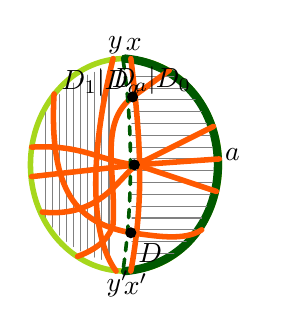
\begin{tikzpicture}[x=.75cm,y=.75cm,line cap=round]
\draw[yellow!65!green,line width=2pt](0,0)ellipse(1.6 and 1.8);
\draw[green!35!black,line width=3pt](0,1.8)..controls(2.1,1.6)and(2.1,-1.6)..(0,-1.8);
\foreach \x in {-1.35,-1.23,...,-.15}{\draw[gray,thin](\x,{1.65*sqrt(1-\x*\x/2.56)})--(\x,{-1.65*sqrt(1-\x*\x/2.56)});}
\foreach \y in {-1.5,-1.3,...,1.5}{\draw[gray,thin](.12,\y)--({1.5*sqrt(1-\y*\y/3.24)},\y);}
\draw[orange!70!red,line width=2pt](-1.2,1.2)..controls(-1.3,-.6)and(-.7,-1)..(.1,-1.15)..controls(.5,-1.2)and(1,-1.3)..(1.3,-1.1);
\draw[orange!70!red,line width=2pt](-.2,1.8)..controls(-.6,.2)and(-.6,-1.2)..(-.15,-1.8);
\draw[orange!70!red,line width=2pt](.1,1.8)..controls(.3,.2)and(.3,-.7)..(.1,-1.8);
\draw[orange!70!red,line width=2pt](-1.58,.3)..controls(-.7,.35)and(-.4,.05)..(.2,0)--(1.55,-.45);
\draw[orange!70!red,line width=2pt](-1.58,-.2)--(.2,0)--(1.6,.1);
\draw[orange!70!red,line width=2pt](-1.4,-.8)..controls(-.4,-.9)and(-.1,-.2)..(.2,0)--(1.5,.65);
\draw[orange!70!red,line width=2pt](-.8,-1.55)..controls(-.4,-1.4)and(-.25,-1.2)..(-.2,-1)..controls(-.15,-.1)and(-.45,.7)..(.13,1.15)--(.75,1.6);
\draw[green!35!black,dashed,line width=1.3pt](-.03,1.77)..controls(.13,.7)and(.14,-.6)..(-.03,-1.77);
\fill(.13,1.15)circle(2pt);\fill(.16,0)circle(2pt);\fill(.1,-1.15)circle(2pt);
\node at(-.16,2.02){$y$};\node at(.15,2.04){$x$};
\node at(-.12,-2.02){$y'$};\node at(.18,-2.02){$x'$};
\node at(-.4,1.4){$\unsure{D_1|D_a}$};\node at(.45,1.43){$\unsure{D_a|D_0}$};
\node at(.43,-1.5){$D$};\node at(1.82,.17){$a$};
\end{tikzpicture}}

mais la configuration obtenue en fait n'est autre que celle de $D$, $\Delta_D$, à isom canonique près. Il est entendu que l'arc $a$ a été tiré jusqu'en $y,y'$, immédiatement adjacents à $x,x'$, le nouvel arc qui est ainsi formé, en pointillés bleus, est \deleted{\unsure{a}} canoniquement isomorphe (en tant que \unsure{graphe-segment} topologique, ou combinatoire) à $a$,

Il est donc tentant de procéder comme tantôt, et de recoller $\Delta_L$ à $\Delta_D$ par cet iso. canonique, qui donne lieu à un isom de transport
\diagram{\begin{tikzcd}[ampersand replacement=\&,row sep=large,column sep=large]
\omega(\Delta_L)\arrow[r]\&\omega(\Delta_D)\\
\omega(L)\arrow[u,phantom,"\rotatebox{90}{$\simeq$}" description]\&\omega(D)\arrow[u,phantom,"\rotatebox{90}{$\simeq$}" description]
\end{tikzcd}}
qui est à nouveau ``\uline{opposé}'' de l'isom tautologique.

L'arc correspondant sur $\Delta_D$ sera appelé arc de générisation. Chaque sommet de $D$ détermine un arc de \uline{générisation}. L'ennui là, c'est que ces arcs de générisation empiètent les uns sur les autres !
